
\subsection{Long range potential: Hierarchical Tree algorithms}
\label{section:intro:md:tree}

The $O\pa{N^2}$ scaling of the MD algorithm for long-range forces
can be problematic when the number of
particles simulated is more than many thousands, which is a potential target
for laser-cluster interaction. Some interesting variations of the MD algorithm
exist to reduce the computational burden. One class of methods uses
\textit{hierarchical tree}
algorithms as introduced by Barnes and Hut in 1986\cite{Barnes1986}. To
reduce the computational burden, particles are grouped in a hierarchical tree
(quadtree in two dimensions, octree in three). While Barnes used his
\textit{treecode} to solve the N-body problem in the context of gravitational
interactions, it can also be applied in the electrostatic case.

The main issue with the direct calculation of forces in MD is the lack of
distinction between the close and distant particles. While the resulting
potential of a distant particle is small, the computational cost required to
calculate it is the same as in the case of a nearby particle. Some MD
calculations use an artificial cutoff: particles farther than this cutoff will
be ignored. This is acceptable
when the force acting on particles is of short range, either due to screening or
to the nature of the force (Lennard-Jones for example).
In the present work, the dominant force is the
Coulomb force and is long range by nature; it thus cannot be artificially
cut off as in the case of close range forces used in other fields.

Could distant particles be grouped together, with their contribution to the
force (or potential) being calculated only once (per ``group'')? Because
individual particles which are part of a distant group will have a similar
contribution to the potential at the location of particle $i$, the interaction
with this group can instead be approximated through the multipole
expansion\cite{Gibbon2002} of the group of particles, or cell in terms of the
tree algorithm:
\begin{align}
\phi_i & = \sum_{j~\textrm{cell}} \phi_{j \rightarrow i} = \sum_{j~{\rm cell}}
\frac{k q_j}{r_{ji}}, \\
& \approx \frac{M_{c}}{R}
+ \sum_{\alpha} \frac{r_{\alpha} D_{c,\alpha}}{R^3}
+ \frac{1}{2} \sum_{\alpha,\beta} \frac{
        Q_{c,\alpha,\beta} r_{\alpha} r_{\beta}
    }{R^5},
\end{align}
where $M_{c}$, $D_{c,\alpha}$ and $Q_{c,\alpha,\beta}$ are the monopole, dipole
and quadrupole moments of the cell defined as:
\begin{subequations}
\begin{align}
M_{c}           ~~~~& = \sum_{j~\textrm{cell}} q_{j}, \\
D_{c,\alpha}      ~~& = \sum_{j~\textrm{cell}} q_{j} r_{j,\alpha}, \\
Q_{c,\alpha,\beta}  & = \sum_{j~\textrm{cell}} q_{j} \pa{3 r_{j,\alpha}
r_{j,\beta} - r_{j}^2} \delta_{\alpha,\beta},
\end{align}
\label{eqn:tree:moments}
\end{subequations}
and $R$ is the distance between the cell's centre-of-charge and the
particle of interest $i$.

\begin{figure}
 \centering
 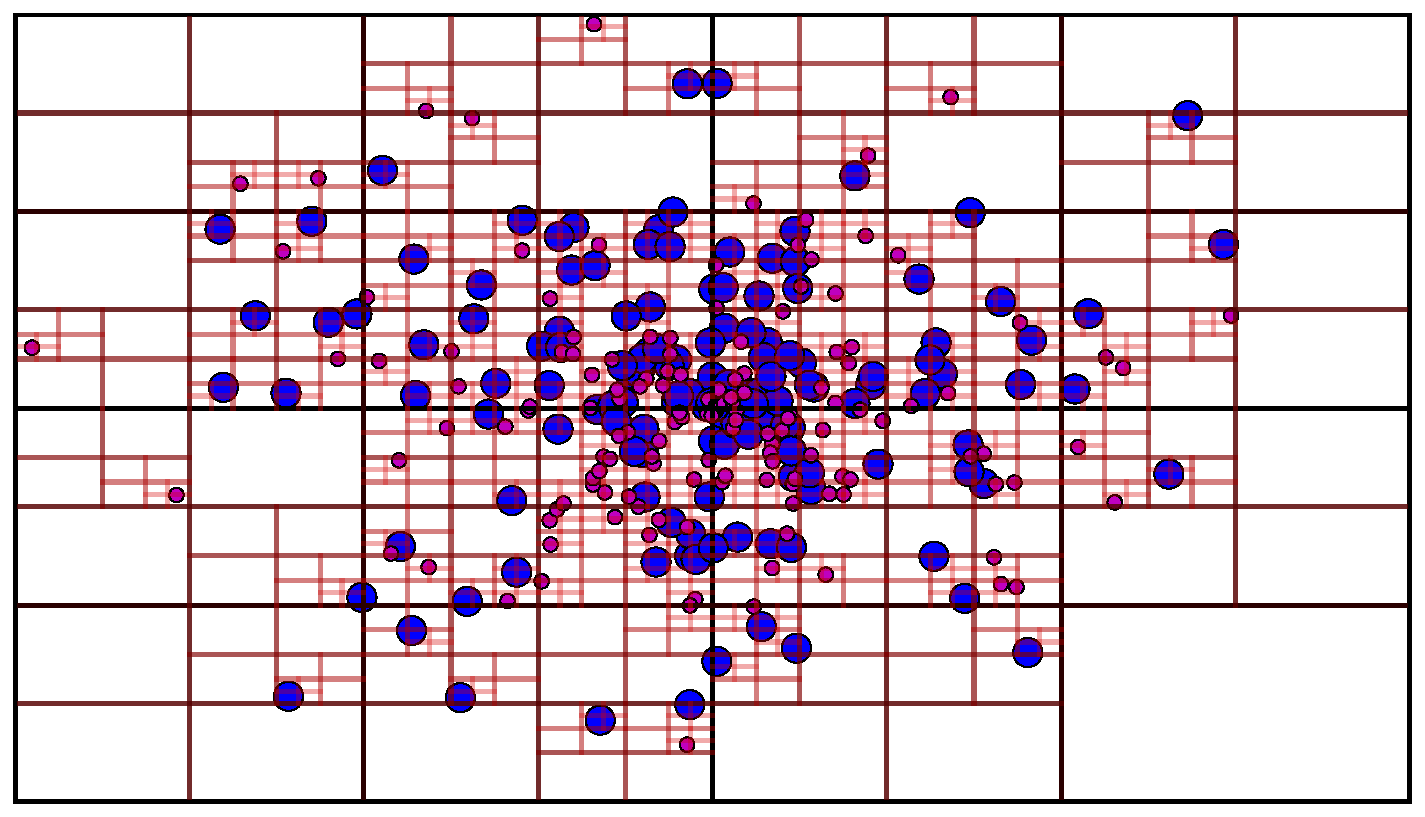
\includegraphics[width=\figurewidth]{figures/quadtree}
 \caption{\label{fig:tree:quadtree}Quadtree: 2D's equivalent of the 3D octree.
          300 particles (half ions in blue, half electrons in magenta) represent
          an exploding cluster. Cells' moments are propagated up the tree to the
          root cell. Particles distant from a cell can interact directly with it
          instead of resolving all particles contained in it, thus reducing the
          computational burden.}
\end{figure}


The tree algorithm first split the computational domain into an octree (in
three dimensions) or quadtree (in two dimensions) until
only a maximum of one particle is present per cell as can be seen figure
\ref{fig:tree:quadtree}. The deepest cells of the tree, containing only one particle,
are called leaves. Once every particle in the system is inserted in the tree,
the electrostatic moments are propagated from the leaves up to the root cell,
the top cell enclosing the whole domain.

Then, instead of iterating through all particles for the calculation of the
force on the particle of interest $i$, the tree is traversed. If the cell is
``far enough'' (with a given definition of far enough, discussed next) it can
be added to the cell interaction list for later processing through the cell's
moments. In the case of
the cell being too close, it must be resolved into its  eight \textit{daughter}
cells (or four in 2D). The daughter cells containing particles are visited, while the empty
ones are ignored. Leaf cells can be reached using this process; in this
case, the particles in the leaves are considered close enough to the particle
of interest $i$ and a direct interaction is wanted. Leaf particles will thus
be added to a second interaction list containing particle-particle direct
interactions. The process is recursively repeated until all particles
are added to an interaction list, either directly or through a parent cell.
Note that an optimization done in the
implementation allows many particles per leaves and automatically adds them
to the particles interaction list when traversing the tree, preventing trees
which are overly unbalanced.

Different selection rules exist for the criteria of ``far enough''. These
rules are called \textit{Multipole Acceptance Criteria} or
MAC\cite{Pfalzner1996}. Barnes' original rule simply referred to as
``\textit{s/d}'' compares an input parameter $\theta$ with the cell's size $s$
divided by the distance between the cell's center-of-charge and particle of
interest $i$ (see figure \ref{fig:tree:mac:1}).
If the ratio $s/d$ is smaller than the parameter $\theta$, the
group of particles contained inside the cell is approximated through the cell's
moments and the cell is added to the cells interaction list. At the opposite, if
the ratio is larger than $\theta$, the cell will be resolved into its daughters.
In the limit where $\theta$ reaches zero, no more cells are added to the
cells interaction list (they are all resolved) and the MD algorithm emerges, though
with a large overhead due to the tree construction and traversal.

Unfortunately, this MAC can cause huge errors when a large amount of charge is
present in a corner of a cell\cite{Pfalzner1996}.
% Page 85 (97), figure 4.13
In this case, a cell could be added to the cell
interaction list even though the error introduced by the multipole expansion is
significant. Different MAC have thus been proposed to mitigate this problem.
The \textit{minimum distance} MAC replaces the distance $d$ in the MAC with the
minimum distance to one of the cell's edge (figure \ref{fig:tree:mac:2}).
The \textit{B-max} MAC instead
replaces the size of the cell with the largest distance between one of the
cell's corner to the center-of-charge (figure \ref{fig:tree:mac:3}).
Another MAC was proposed by
B\'edorf~\textit{et.~al.}~\cite{Bedorf2012} and is a mix of the two previous.
The MAC reads:
\begin{align}
d > \frac{s}{\theta} + \delta,
\end{align}
where $\delta$ is the distance between the cell's geometric center and its
center-of-charge (figure \ref{fig:tree:mac:4}).
If the previous equation holds ($d$ is large enough) then the
multipole expansion is used and the cell is added to the interaction list.

\begin{figure}
 \centering
    \begin{subfigure}{0.15\columnwidth}
        \centering
        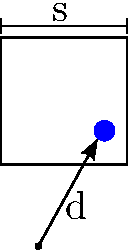
\includegraphics[width=\textwidth]{figures/mac_1}
        \caption{ $s/d$}
        \label{fig:tree:mac:1}
    \end{subfigure}
    \hspace{0.75cm}
    \begin{subfigure}{0.15\columnwidth}
        \centering
        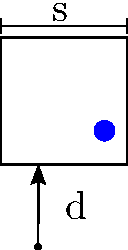
\includegraphics[width=\textwidth]{figures/mac_2}
        \caption{min. $d$}
        \label{fig:tree:mac:2}
    \end{subfigure}
    \hspace{0.75cm}
    \begin{subfigure}{0.15\columnwidth}
        \centering
        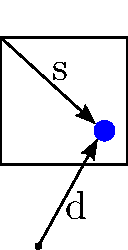
\includegraphics[width=\textwidth]{figures/mac_3}
        \caption{B-max}
        \label{fig:tree:mac:3}
    \end{subfigure}
    \hspace{0.75cm}
    \begin{subfigure}{0.15\columnwidth}
        \centering
        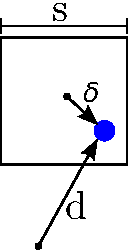
\includegraphics[width=\textwidth]{figures/mac_4}
        \caption{Bédorf\cite{Bedorf2012}}
        \label{fig:tree:mac:4}
    \end{subfigure}
\caption{Different Multipole Acceptance Criteria (MAC). See text for descriptions.}
\label{fig:tree:mac}
\end{figure}


Because not all interaction pairs are considered in the calculation of the
force and potential in this tree algorithm,
a significant speedup is obtained. Due to the tree
traversal algorithm, the scaling improves
from $O\pa{N^2}$ to $O\pa{N \log{N}}$\cite{Barnes1986,Gibbon2002,Pfalzner1996}.

A variation of the hierarchical treecode is obtained when a sufficiently large
$\theta$ is used. In this case, the root cell (the largest one) is never
resolved into its daughters. By adding more moments to the approximation then
the first three of equations \eqref{eqn:tree:moments} and removing
contributions of nearby particles, the \textit{Fast Multipole Method} (FMM) is
obtained\cite{Pfalzner1996}. FMM was developed by Greegard in
1988\cite{Greengard1987} independently of Barnes' hierarchical tree method.
While conceptually similar, its implementation details are quite different and
it has not been implemented in the current work while the hierarchical tree
algorithm was.

